%; whizzy chapter -dvi
% -initex iniptex -latex platex -format platex -bibtex jbibtex -fmt fmt
% 以上 whizzytex を使用する場合の設定。
 
%     Tokyo Debian Meeting resources
%     Copyright (C) 2012 Junichi Uekawa
%     Copyright (C) 2011, 2015 Nobuhiro Iwamatsu

%     This program is free software; you can redistribute it and/or modify
%     it under the terms of the GNU General Public License as published by
%     the Free Software Foundation; either version 2 of the License, or
%     (at your option) any later version.

%     This program is distributed in the hope that it will be useful,
%     but WITHOUT ANY WARRANTY; without even the implied warranty of
%     MERCHANTABILITY or FITNESS FOR A PARTICULAR PURPOSE.  See the
%     GNU General Public License for more details.

%     You should have received a copy of the GNU General Public License
%     along with this program; if not, write to the Free Software
%     Foundation, Inc., 51 Franklin St, Fifth Floor, Boston, MA  02110-1301 USA

%  preview (shell-command (concat "evince " (replace-regexp-in-string "tex$" "pdf"(buffer-file-name)) "&"))

%%ここからヘッダ開始。

\documentclass[mingoth,a4paper]{jsarticle}
\usepackage{monthlyreport}
% 日付を定義する、毎月変わります。
\newcommand{\debmtgyear}{2016}
\newcommand{\debmtgmonth}{2}
\newcommand{\debmtgdate}{13}
% started from zero:
% (let ((year 2013) (month 7)) (+ (* (- year 2005) 12) month -1))
\newcommand{\debmtgnumber}{136}

\begin{document}

\begin{titlepage}
\thispagestyle{empty}
% タイトルページ:編集必要な部分は最初のマクロに飛ばすこと

\vspace*{-2cm}
第\debmtgnumber{}回 東京エリア Debian 勉強会資料\\
\hspace*{-2cm}

\includegraphics{image2012-natsu/dotdeb.pdf}\\
\hfill{}\debmtgyear{}年\debmtgmonth{}月\debmtgdate{}日

% ここはアップデートすること
% 全角文字にしないとフォントのサイズが合わないので注意
\rotatebox{10}{\fontsize{30}{30} {\gt 特集 :Debianの消費電力管理}}\\

\vspace*{-2cm}
\hfill{}
\includegraphics[height=6cm]{image200502/openlogo-nd.eps}
\end{titlepage}

\newpage

\begin{minipage}[b]{0.2\hsize}
 \definecolor{titleback}{gray}{0.9}
 \colorbox{titleback}{\rotatebox{90}{\fontsize{80}{80} {\gt デビアン勉強会} }}
\end{minipage}
\begin{minipage}[b]{0.8\hsize}
\hrule
\vspace{2mm}
\hrule
\begin{multicols}{2}
\tableofcontents
\end{multicols}
\vspace{2mm}
\hrule
\end{minipage}

\dancersection{事前課題}{野島 貴英}

今回の事前課題は以下です:
\begin{enumerate}
\item hack time に何をしますか?
\item 本勉強会をどこでお知りになりましたか?(任意回答) 
\end{enumerate}
この課題に対して提出いただいた内容は以下です。
\begin{multicols}{2}
{\small
\begin{prework}{ takaswie }
  \begin{enumerate}
  \item Q.hack time に何をしますか?\\
    A.hinawa-utils の開発。あるいはALSAの開発。\\
https://github.com/takaswie/hinawa-utils
  \item Q.本勉強会をどこでお知りになりましたか?(任意回答)\\
    A. ML
  \end{enumerate}
\end{prework}


\begin{prework}{ mkouhei }
  \begin{enumerate}
  \item Q.hack time に何をしますか?\\
    A.
    \begin{itemize}
    \item https://qa.debian.org/developer.php? login=mkouhei@palmtb.net のメンテ。
    \item パッケージ ( https://qa.debian.org/developer.php? login=mkouhei@palmtb.net ) のメンテナンス
    \item keybase.io を signing-party( caff ) のキーサーバーとして利用できないかの検証

   \end{itemize}
    \item Q.本勉強会をどこでお知りになりましたか?(任意回答)\\
    A. 常連
   \end{enumerate}
\end{prework}

\begin{prework}{ Poeto }
  \begin{enumerate}
  \item Q.hack time に何をしますか?\\
    A.「 Debian 」 の基本操作。( 数日前、インストールしたばかりなので )
  \item Q.本勉強会をどこでお知りになりましたか?(任意回答)\\
    A. Web
  \end{enumerate}
\end{prework}

\begin{prework}{ kenhys }
  \begin{enumerate}
  \item Q.hack time に何をしますか?\\
    A. 未定。
  \item Q.本勉強会をどこでお知りになりましたか?(任意回答)\\
    A. ML
  \end{enumerate}
\end{prework}

\begin{prework}{ iwamatsu }
  \begin{enumerate}
  \item Q.hack time に何をしますか?\\
    A. package メンテナンス。
  \item Q.本勉強会をどこでお知りになりましたか?(任意回答)\\
    A. ML
  \end{enumerate}
\end{prework}

\begin{prework}{ Charies }
  \begin{enumerate}
  \item Q.hack time に何をしますか?\\
    A. パッケージング。
  \end{enumerate}
\end{prework}

\begin{prework}{ dictoss }
  \begin{enumerate}
  \item Q.hack time に何をしますか?\\
    A. kfreebsd の Intel GPU ビデオドライバのデバッグ( unstable で動かなくなった)
  \item Q.本勉強会をどこでお知りになりましたか?(任意回答)\\
    A. Web
  \end{enumerate}
\end{prework}

\begin{prework}{ rosh }
  \begin{enumerate}
  \item Q.hack time に何をしますか?\\
    A. d-i に関する作業
  \item Q.本勉強会をどこでお知りになりましたか?(任意回答)\\
    A. twitter
  \end{enumerate}
\end{prework}

\begin{prework}{ wskoka }
  \begin{enumerate}
  \item Q.hack time に何をしますか?\\
    A. tilegx
  \end{enumerate}
\end{prework}

\begin{prework}{ yy\_y\_ja\_jp }
  \begin{enumerate}
  \item Q.hack time に何をしますか?\\
    A. DDTSS
  \end{enumerate}
\end{prework}

\begin{prework}{ 野島 }
  \begin{enumerate}
  \item Q.hack time に何をしますか?\\
    A. DDTSS、xmrisパッケージ化など。
  \item Q.本勉強会をどこでお知りになりましたか?(任意回答)\\
    A. 幹事なので!\\ところでセミナか、幹事やってみたい人はいつでも募集中!\\貴殿好みの勉強会にしてくれてもよくてよ!
  \end{enumerate}
\end{prework}


}
\end{multicols}

\dancersection{Debian Trivia Quiz}{野島 貴英}

Debianの昨今の話題についてのQuizです。

今回の出題範囲は\url{debian-devel-announce@lists.debian.org} や \url{debian-news@lists.debian.org}に投稿された
内容などからです。

\begin{multicols}{2}
%; whizzy-master ../debianmeetingresume201311.tex
% $B0J>e$N@_Dj$r$7$F$$$k$?$a!"$3$N%U%!%$%k$G(B M-x whizzytex $B$9$k$H!"(Bwhizzytex$B$,MxMQ$G$-$^$9!#(B
%

\santaku
{2016/2/3$B$K$F!"(Bdebtag$B$N(Btag$BIU$1$K$D$$$F$NJQ99$,N.$l$^$7$?!#0J2<$N$I$l!)(B}
{tag$BIU$1GQ;_(B}
{tag$BIU$1$K$D$$$F%f!<%6G'>ZIU$-$K$9$k(B}
{tag$B$N%l%S%e!<$r$5$i$K6/8G$K$9$k(B}
{B}
{debtag$B$rJT=8$G$-$k%5%$%H$,$$$m$$$m%j%K%e!<%"%k$9$k$H$$$&%"%J%&%s%9$,N.$l!"<B:]$$$/$D$b<B9T$5$l$?$h$&$G$9!#$^$:!"F?L>$K$h$k(Btag$BIU$1$NJT=8$rGQ;_$7!"Be$o$j$K(Bsso.debian.org$B$K$h$k%7%s%0%k%5%$%s%*%s$G%f!<%6G'>Z$7$J$$$HJT=8=PMh$J$$$h$&$K$7$?$H$N$3$H!#$^$?!"(Btag$BJT=8$N(BURL$B$,JQ99$K$J$C$F$*$j!"(Bhttps://debtags.debian.org/$B$H$J$j$^$7$?!#B>$K$b$$$m$$$mJQ99$,=P$F$$$^$9$N$G!">\$7$/$O(Bhttps://lists.debian.org/debian-devel-announce/2016/02/msg00000.html $B;2>H!#(B}

\santaku
{2016/1/12$B$K$F!"(Bdebian sid$B$K(Bphp$B$N?7$7$$%P!<%8%g%s$rF~$l$?7o$,%"%J%&%s%9$5$l$^$7$?!#$I$N%P!<%8%g%s!)(B}
{php 7.0}
{php 5.6}
{php$B$C$F2?!)(B}
{A}
{php7.0$B$,(Bdebian sid$B$K$F%j%j!<%9$5$l$^$7$?!#$A$J$_$K!"(Bphp7$B$NL\6L5!G=$OBgI}$J<B8zB.EY2~A1$G$9!#$3$l$G<!4|0BDjHG%P!<%8%g%s$G$"$k(Bstrech$B$G!"(Bphp7$B$,MxMQ$G$-$k8+9~$_$,$H$F$b9b$/$J$C$F$-$^$7$?$M!*(B}

\santaku
{dbgsym$B%Q%C%1!<%8$G$9$,!"$3$A$i$rJ]4I$9$k%_%i!<@h$O$I$3$G$7$g$&!)(B}
{mirrors.debian.org}
{debug.mirrors.debian.org}
{ftp.jp.debian.org}
{B}
{debhelper 9.20151219$B0J9_$K$F!">o$K%G%P%C%0MQ%7%s%\%k$r<}$a$?%Q%C%1!<%8!JL>A0$O%Q%C%1!<%8L>(B-dbgsym)$B$r@8@.$9$k$h$&$K$J$j$^$7$?!#$3$N(B-dbgsym$B%Q%C%1!<%8$NJ]4I@h$,%"%J%&%s%9$5$l!"(Bhttp://debug.mirrors.debian.org/debian-debug/$B$H!"(Bhttp://snapshot.debian.org/archive/debian-debug/$B$K$J$C$?$h$&$G$9!#(B}


\end{multicols}


\dancersection{最近のDebian関連のミーティング報告}{野島 貴英}

\subsection{第135回東京エリアDebian勉強会}

 今回場所はdotsさんをお借りしての開催でした。参加者は10名でした。

 セミナ内容は、2本建てで、
  \begin{enumerate}
  \item 参加者皆さんによる「 Debian 今年の半年分の計画を立ててみた 」
  \item 野島さんによる「 Debian で Linux Ftrace まわりをいじってみた  」
  \end{enumerate}
でした。残りの時間でhack timeを行い、成果発表をしました。

 「Debian 今年の半年分の計画を立ててみた」は、2016年6月末までのDebianプロジェクトで行う目標を書いて頂きました。みなさん、がっちり目標を立てていただけました。あとは、実行あるのみですね。

 「Debian で Linux Ftrace まわりをいじってみた」は、linux kernelに搭載されているデバッグI/FであるFtraceをDebianで利用してみた事について語られました。Debian sidに搭載されているkernelが4.3.3であることから、USDTを利用してみたり、kprobeを利用した話をしました。Debianに搭載されているFtrace利用のツールである、perf-toolが古かった件についても、BUG Report\footnote{https://bugs.debian.org/813769}が行われました。

  また、hack timeですが、成果をtitanpad.comに記載する試みを行いました。
 表は前回のhack time中の成果の一覧となります。(敬称略)

\begin{table}
\begin{center}
  \begin{tabular}{|l|p{15cm}|}
    \hline
参加者 & 成果 \\ \hline \hline
henrich &   proposal for Debian idea
  \begin{itemize}
  \item integrate piuparts into repository pipeline
  \item replace dput $\rightarrow$ lintian + piuparts, then upload
   + prevents regression into repository
  \end{itemize} \\ \hline
kenhys & libhinawaのdebian/*に手をいれていくつかPRを投げたり、issueを立てたりした。参考:
\begin{itemize}
\item \url{https://github.com/takaswie/libhinawa/pull/20}
\item \url{https://github.com/takaswie/libhinawa/pull/21}
\item \url{https://github.com/takaswie/libhinawa/pull/24}
\end{itemize}\\ \hline
tai &   \begin{itemize}
    \item キーサインを行った。 caffではなく手動で。
    Keysigning with the GNU/Linux Terminal(
    \url{http://www.phillylinux.org/keys/terminal.html})
    に沿ってやってみた。しかし最後の署名したキーを送る所がGmail経由になり署名・暗号化せずに返送してしまったので、caffがやっぱりいいのか・・・
  \item Debian Wikiの翻訳し残しの続きをもくもくと。
  \end{itemize} \\ \hline
wskoka &   tilegx用パッケージ作成(10こぐらい。トータルは1200個ぐらいある。)\\ \hline
rosh &
  \begin{itemize}
  \item caff でキーサインが出来た
  \item 前マージされたLinkstation DTS [0] をベースにて、新Linkstationデバイス (LS-QVL)の DTS を別のユーザ様が出来たとの連絡がありました。今週受け入れられた Linkstation DTS [1] にマージを行いました。これから ARM kernel lists にアップする予定です。
    \begin{enumerate}
    \item Kernel tree: arch/arm/boot/dts/kirkwood-{lswvl,lswxl}.dts
    \item \url{http://lists.infradead.org/pipermail/linux-arm-kernel/2016-January/400949.html}
    \end{enumerate}
  \end{itemize} \\ \hline
dictoss &   \begin{itemize}
  \item rasberry pi2のdebian jessieからbluetoothテザリングできた
  \item キーサインしました
  \item 東京エリアDebian勉強会のwebサイトをHTML5対応とスマートフォン対応作業(リポジトリの場所確認、ソースコードを読んで中身と作りを把握中)\footnote{2016年2月27日に無事リリースされ、tokyodebian.alioth.debian.orgは、祝!モバイルフレンドリーになりました!}
  \end{itemize} \\ \hline
y.y &
  \begin{itemize}
   \item 参加者とkey signを行った。
   \item Caffで、溜まっていた keysigning 処理のキューをフラッシュできた。
  \end{itemize} \\ \hline
  \end{tabular}
\end{center}
\caption{hack time成果}
\end{table}

\begin{table}
\begin{center}
  \begin{tabular}{|l|p{15cm}|}
    \hline
参加者 & 成果 \\ \hline \hline
takaswie & 
 Echo Audio Corp.のFireworksデバイスモジュール向けコマンドラインツールがだいたい書けた。
\url{https://github.com/takaswie/hinawa-utils} \\ \hline
yy\_y\_ja\_jp & 
  \begin{itemize}
  \item uim-qt5 バグレポート
  \item キーサイン
  \item DDTSS
  \end{itemize} \\ \hline
野島 &9個のDDTSSのレビューを行いました。なお、yorickはtypoの''M-x Yorick''を見落とし、requeueしました。\\ \hline
  \end{tabular}
\end{center}
\caption{hack time成果(つづき)}
\end{table}

% % (query-replace-regexp "<.*?>" "")
% % (query-replace-regexp "^[	 ]\+" "")

%-------------------------------------------------------------------------------
\dancersection{Debian GNU/Linux 上での省電力設定について}{岩松}
%-------------------------------------------------------------------------------

\subsection{はじめに}

Linux がインストールされたノートPCを利用している時、スペック通りにバッテリが持たない場合が多々あります。
数年前と比べると Linux 上の電源管理対応も進んでいますが、まだWindowsなどのOSにはまだまだ及ばないところがあります。
とは言ってもデフォルトの状態で使うより、少しパラメータを操作してみたり、管理用のツールをインストールするだけで
バッテリの持ちはよいものなります。少しでもDebian でのノートPCライフを過ごすために 今回は Debian GNU/Linux を題材に
した 省電力設定方法について説明します。


\subsection{省電力設定するためには}

省電力設定するためにはどのような点で電力を消費しているのかを簡単に理解しておくことが重要です。
Linux の場合、大きく分けて以下の点が重要となってきます。

\begin{itemize}
\item CPUと制御
\item 動作しているデバイス
\item 動作しているプログラム
\end{itemize}

これらについて、Debianでの対応方法について簡単に説明します。

\subsubsection{CPUと制御}

CPUですが、Intel製CPUのCPU状態遷移は図\ref{fig:cpustate}のようになっており、CPU稼働状態と
スリープ状態の切り替えが頻繁に行われています。CPUにはステート(Cステート)という状態があり、
この状態によって消費電力が異なり、CPUの復帰時間も変わってきます。最新のCPUではもっと細かいステートが提供
されるようになっています。これらを制御しているのがACPIとなります。

\begin{figure}[H]
\begin{center}
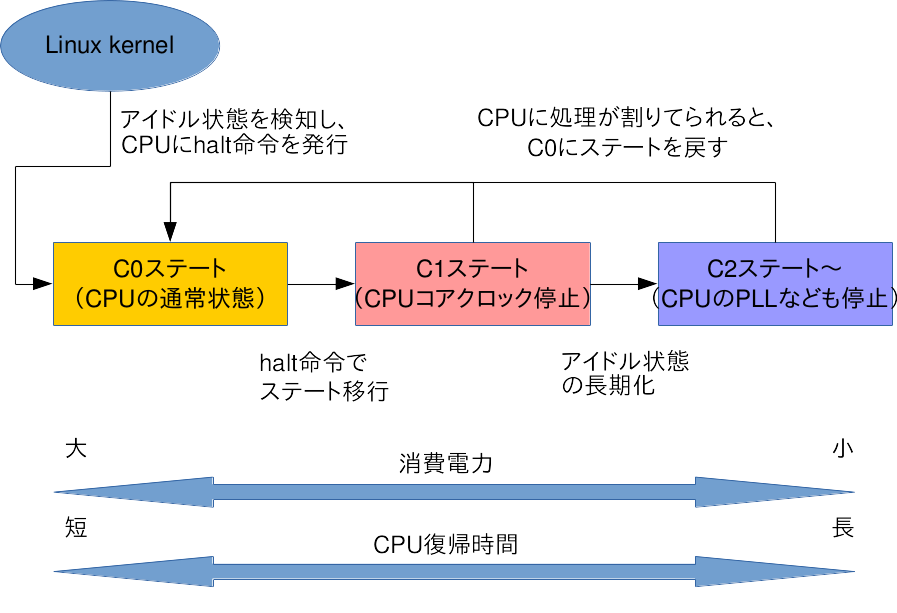
\includegraphics[width=0.5\hsize]{image201602/cpustate.png}
\end{center}
\label{fig:cpustate}
\caption{CPU状態遷移簡易図} 
\end{figure}

実際のCPUはCステートだけではなく、CPUの電圧やクロック数なども関連してきます。
Linux の場合はCPU周波数スケーリング機能を使うことで、OSが自動的に制御できるようになっています。
これは Linux カーネルの cpufreq によって実装されています。
現在の cpufreq に設定されている内容を確認するには cpufrequtils パッケージで提供されている
cpufreq-info(\ref{fig:cpufreq-info}) コマンドを使います。

\begin{figure}[htbp]
\begin{commandline}
$ cpufreq-info
cpufrequtils 008: cpufreq-info (C) Dominik Brodowski 2004-2009
Report errors and bugs to cpufreq@vger.kernel.org, please.
analyzing CPU 0:
  driver: intel_pstate
  CPUs which run at the same hardware frequency: 0
  CPUs which need to have their frequency coordinated by software: 0
  maximum transition latency: 0.97 ms.
  hardware limits: 800 MHz - 2.90 GHz
  available cpufreq governors: performance, powersave
  current policy: frequency should be within 800 MHz and 2.90 GHz.
                  The governor "powersave" may decide which speed to use
                  within this range.
  current CPU frequency is 1.90 GHz.
....
\end{commandline}

\caption{cpufreq-info 実行結果}
\label{fig:cpufreq-info}
\end{figure}

いくつか項目がありますが、重要となるのは 「available cpufreq governors」と
「current policy」です。
available cpufreq governors は CPUの調整可能な速度調整名(ガバナー)であり、
以下のものが用意されています。

\begin{table}[htb]
\begin{center}
\begin{tabular}{l|l}
ガバナー & 内容 \\
ondemand &	CPU負荷が大きい、または小さい時にCPUクロックを大きくに切り替える \\
conservative &	CPU負荷が大きい、または小さい時にCPUクロックを徐々に切り替える \\
performance &	最大周波数でCPUを動作させる \\
powersave &	最小周波数でCPUを動作させる \\
userspace &	ユーザーが指定した周波数でCPUを動作させる \\
\end{tabular}
\caption{指定できるガバナー}
\label{tab:governors}
\end{center}
\end{table}

これらは実際には設定できる値カーネルや環境によって異なる点に注意が必要です。
「current policy」は現在設定されているガバナーが表示されます。

この以上から、上記の結果では

\begin{itemize}
\item CPUが800MHzから2.90GHzまでをサポートしている
\item powersave governor で動作している
\item 最大値と最小値のポリシー設定により、800MHzから2.90GHzの間で変動させている
\end{itemize}

ということがわかります。

これらを設定するには sysfs 経由で操作するか、cpufrequtils に含まれる
cpufreq-set コマンドを使います。

\begin{itemize}
\item ガバナーを設定する
  \begin{commandline}
   $ sudo cpufreq-set -c CPU番号 -g ガバナー名
   または
   $ sudo sh -c "echo ガバナー名 > /sys/devices/system/cpu/cpuCPU番号/cpufreq/scaling_governor"
  \end{commandline}

\item 最小クロックを設定する
  \begin{commandline}
   $ sudo cpufreq-set -c CPU番号 -d クロック値
   または
   $ sudo sh -c "echo クロック値 > /sys/devices/system/cpu/cpuCPU番号/cpufreq/scaling_min_freq"
  \end{commandline}

\item 最大クロックを設定する
  \begin{commandline}
   $ sudo cpufreq-set -c CPU番号 -u クロック値
   または
   $ sudo sh -c "echo クロック値 > /sys/devices/system/cpu/cpuCPU番号/cpufreq/scaling_max_freq"
  \end{commandline}

\item 現在のクロックを設定する
  \begin{commandline}
   $ sudo cpufreq-set -c CPU番号 -f クロック値
   または
   $ sudo sh -c "echo クロック値 > /sys/devices/system/cpu/cpuCPU番号/cpufreq/scaling_cur_freq"
  \end{commandline}

\end{itemize}

上記のようにしてCPUクロックを制御することにより、環境によって無駄なくCPUを利用できるようになります。
設定した値は再起動すると消えるので、/etc/sysfs.conf に設定しておくか、cpufreq を設定するデーモン cpufreqd
を使うとよいでしょう。

\subsubsection{動作しているデバイスの設定}

使っている個々のデバイスの設定も重要となります。例えば無線LANやBluetoothを使わないのに有効にしていると
それだけで電力を消費してしまいます。よって使用する環境に応じてこれらを制御する必要が出てきます。

ここではよく利用されるデバイスに対する制御方法について説明します。

\begin{itemize}

\item ラップトップモード

Linux の場合はカーネルのモードとして、ラップトップモードが設定できるようになっています。
これは以下のようにして設定します。

\begin{commandline}
$ sudo sh -c "echo 5 > /proc/sys/vm/laptop_mode"
\end{commandline}

あとNMI のwatchdog(nmi\_watchdog) も無効化しておきます。これはこれはカーネルハングアップを定期的にチェックする機構
をコントロールするフラグです。

\begin{commandline}
$ sudo sh -c "echo 0 > /proc/sys/kernel/nmi_watchdog"
\end{commandline}

\item USB

USB は /sys/bus/usb/devices/ 以下に対して設定を行います。
例えば、/sys/bus/usb/devices/usb1 に対して 電源供給を切りたい場合は /sys/bus/usb/devices/usb1/power/control
をoff に設定します。自動的にサスペンドさせたい場合には 
/sys/bus/usb/devices/usb1/power/autosuspend に対して 1 を設定します。

\begin{commandline}
$ sudo sh -c "echo off > /sys/bus/usb/devices/usb1/power/control"
$ sudo sh -c "echo auto > /sys/bus/usb/devices/usb1/power/autosuspend"
\end{commandline}

設定を起動時に適用したい場合は、再起動時に初期化されてしまう事とデバイスのUSB位置が変わる事が
ありますので、 udev の rules ファイルを使って設定するのがよいでしょう。

\begin{commandline}
$ cat /etc/udev/rules.d/70-my-usb-power.rules
ACTION=="add", SUBSYSTEM=="usb", ATTRS{idVendor}=="0x046d", ATTR{idProduct}=="0x08cb", TEST=="power/control", ATTR{power/control}="off"
\end{commandline}

注意しなければいけない点としてはUSBをなんでも設定してしまうとキーボードが動作しなくなる可能性もあるため、
ベンダーID、デバイスIDなどを確認した上で設定しましょう。

\item 無線LAN

無線LANは iw パッケージに含まれる iw コマンドを使って設定します。
無線LANがwlan0の場合は 以下のように設定することによって制御できます。

\begin{commandline}
$ sudo iw dev wlan0 set power_save on
\end{commandline}

これもudev の rules ファイルを使って設定すると良いです。

\begin{commandline}
$ cat /etc/udev/rules.d/70-my-wifi-power.rules
ACTION=="add", SUBSYSTEM=="net", KERNEL=="wlan*", RUN+="/usr/bin/iw dev %k set power_save on"
\end{commandline}

\item サウンド

サウンドの場合も sysfs 経由で設定します。ドライバによって設定出来ない場合がありますが、INTEL のサウンド
コントローラの場合は、power\_save があるので、これを1に設定することによってパワーセーブモードに設定できます。

\begin{commandline}
$ sudo sh -c "echo 1 > /sys/module/snd_hda_intel/parameters/power_save"
\end{commandline}

\item PCI/PCI-Express

PCI/PCI-Express の省電力に設定するには power/control を auto に設定します。
この場合も sysfs 経由で設定します。PCIもUSBと同様に設定先がどのようなデバイス
なのか確認してから設定するようにしましょう。

\begin{commandline}
$ sudo sh -c "echo auto > /sys/bus/pci/devices/0000:00:00.0/power/control"
\end{commandline}

\end{itemize}

\subsubsection{動作しているプログラムについて}

動作しているプログラムはtopコマンドなのでざっくりとしたCPU占有率を確認できますが、実際に
どれぐらいの頻度で使われてているのかわかりません。アイドル状態であるにもかかわらず、CPU割り込みが多い
プログラム・プロセスが省電力の効果が得にくいものとなりますので、このようなプログラム・プロセスを
調べる必要があります。これらを調べるには下記で説明する PowerTop を使うとようでしょう。

\subsection{省電力設定するためのツール}

先では長々と書きましたが、知識がないユーザが上記を一つづつやっていくのは非常に大変です。
Linux では専門の知識がなくとも使っているマシンを省電力状態に設定できるツールがいくつか
準備されています。以下ではそれらの使い方について紹介します。

\subsubsection{PowerTOP}

PowerTOP はIntelが開発しているソフトウェアで、カーネル、ハードウェア、ユーザランドで制御可能な省電力項目を
有効にするツールです。プロセスを監視して、CPU負荷やデバイスドライバの使用状況のレポートからプロセスの操作
を行う事ができます。

\begin{enumerate}

\item インストール

PowerTOP はDebian でも提供されており、apt でインストールできます。
\begin{commandline}
% sudo apt-get install powertop	
\end{commandline}

\item 起動

起動すると図\ref{fig:powertop0}のような画面が表示されます。
「The battery reports a discharge rate ...」 に現在の消費電力が
表示され、現在動作しているプロセスと使用状況がわかります。
筆者の環境で、何も設定しない場合は 13Wのようです。

\begin{figure}[H]
\begin{center}
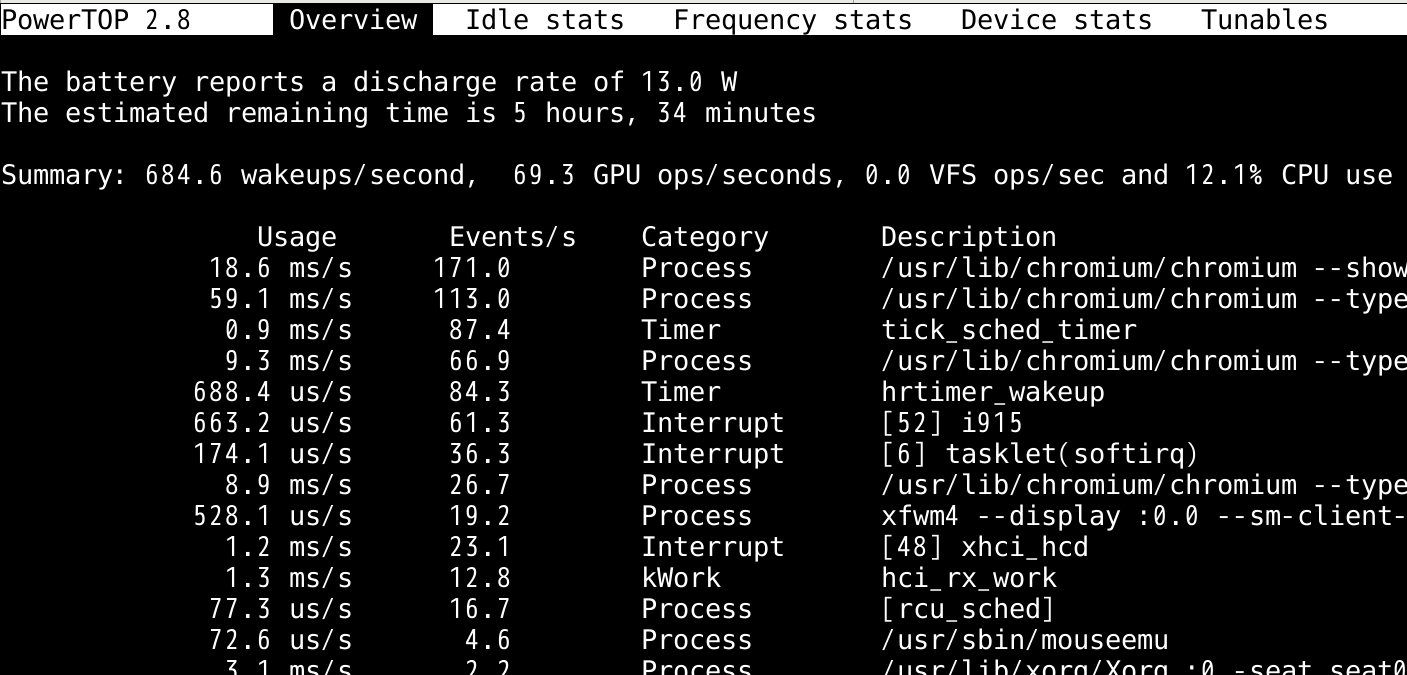
\includegraphics[width=0.5\hsize]{image201602/powertop_00.png}
\end{center}
\label{fig:powertop0}
\caption{PowerTOP起動画面} 
\end{figure}

Tunables タブを選択すると調整可能なシステムの設定が表示されます。
Badが省電力に有効な項目にもかかわらず無効な設定、
Good が既に有効になっている設定となっています。

\begin{figure}[H]
\begin{center}
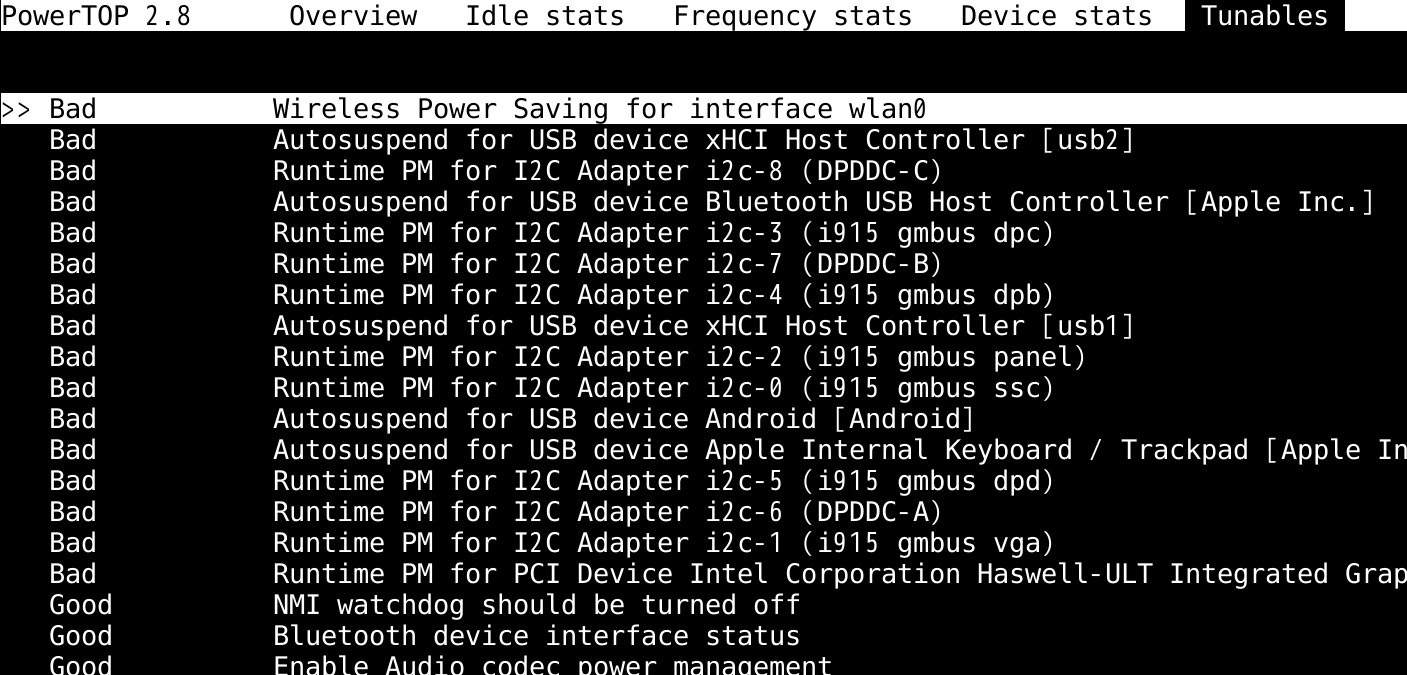
\includegraphics[width=0.5\hsize]{image201602/powertop_01.png}
\end{center}
\label{fig:powertop1}
\caption{Tunables画面} 
\end{figure}

この状態ではまだシステムに最適化された設定になっていないため、一度終了し、
キャリブレーションを行います。

\item キャリブレーション

設定するPCの状態を取得するためにキャリブレーションを行います。
実行するとデバイスなどから使用状況を読み取り、マシンに対して適切な設定を
行います。
ノートPCの場合はいきなりモニターのバックライトが消えるので注意しましょう。

\begin{commandline}
$ sudo powertop --calibrate
\end{commandline}

キャリブレーションが終わると、\texttt{/var/cache/powertop/saved\_parameters.powertop}
以下にデータが保存されます。次回のPowerTOP起動時からはキャリブレーションデータを元に
省電力にされた環境で起動します。

\item キャリブレーション後

キャリブレーション後に起動すると、
「The battery reports a discharge rate ...」 の項目に表示される消費電力値が変わり、システム
全体で省電力で稼働していることが確認できるでしょう。

\item PowerTOP の起動時有効化

PowerTOP は起動すると保存されている設定を元に省電力状態にしてくれますが、PCを立ち上げるたびに
PowerTOP自体を立ち上げる必要があります。

起動時に自動的にPowerTOP を立ち上げるようにするには、以下のように systemd の ユニットファイル
を用意し、有効にしておきます。

\begin{commandline}
$ cat /etc/systemd/system/powertop.service

[Unit]
Description=PowerTOP

[Service]
Type=oneshot
ExecStart=/usr/bin/powertop
Environment="TERM=xterm"

[Install]
WantedBy=multi-user.target
\end{commandline}

\begin{commandline}
$ sudo systemctl enable powertop
\end{commandline}

\end{enumerate}

\subsubsection{TLP を使った設定}

PowerTOP の他にTLPというツールもあります。これは PowerTOPのように詳細なレポートは
出してくれませんが、AC接続時などの状況に応じたスクリプトが準備されており、インストール
するだけである程度省電力設定を行ってくれる便利なツールです。
もちろん、Debian ではパッケージ化されており、apt でインストールできます。

\begin{commandline}
$ sudo apt-get install tlp
\end{commandline}

無線LANの設定等に NetworkManager を使っているなら tlp-rdw パッケージもインストールしておくと
無線LAN、Bluetooth関連の設定も行ってくれます。
デフォルトの設定は /etc/default/tlp にあり、このファイルを変更して環境に合わせた省電力設定を
行います(図\ref{fig:TLP})。設定はよく使われる項目しかなく、使っている環境の設定がない場合もあります。このような場合は
T自分で設定を追加するか、先に説明したようにsysfs / procfs 経由
の設定を別途行う必要があります。


\begin{figure}[H]
\begin{center}
\begin{commandline}
# Set to 0 to disable, 1 to enable TLP.
TLP_ENABLE=1

# Operation mode when no power supply can be detected: AC, BAT
# Concerns some desktop and embedded hardware only.
TLP_DEFAULT_MODE=AC

# Seconds laptop mode has to wait after the disk goes idle before doing a sync.
# Non-zero value enables, zero disables laptop mode.
DISK_IDLE_SECS_ON_AC=0
DISK_IDLE_SECS_ON_BAT=2

# Dirty page values (timeouts in secs).
MAX_LOST_WORK_SECS_ON_AC=15
MAX_LOST_WORK_SECS_ON_BAT=60
...
\end{commandline}
\end{center}
\label{fig:TLP}
\caption{/etc/default/tlp 例} 
\end{figure}

TLP は systemd やその他init用の起動ファイルが用意されているのでPC起動時に設定が反映されるのも
良い点です。

\subsubsection{省電力設定後}
図\ref{fig:powertop2}が省電力設定した後に PowerTOP で消費電力を確認した内容です。
消費電力が13W から 11W に下がっていることがわかります。またPC稼働時間も5時間半から6時間50分に
伸びていることがわかります。

\begin{figure}[H]
\begin{center}
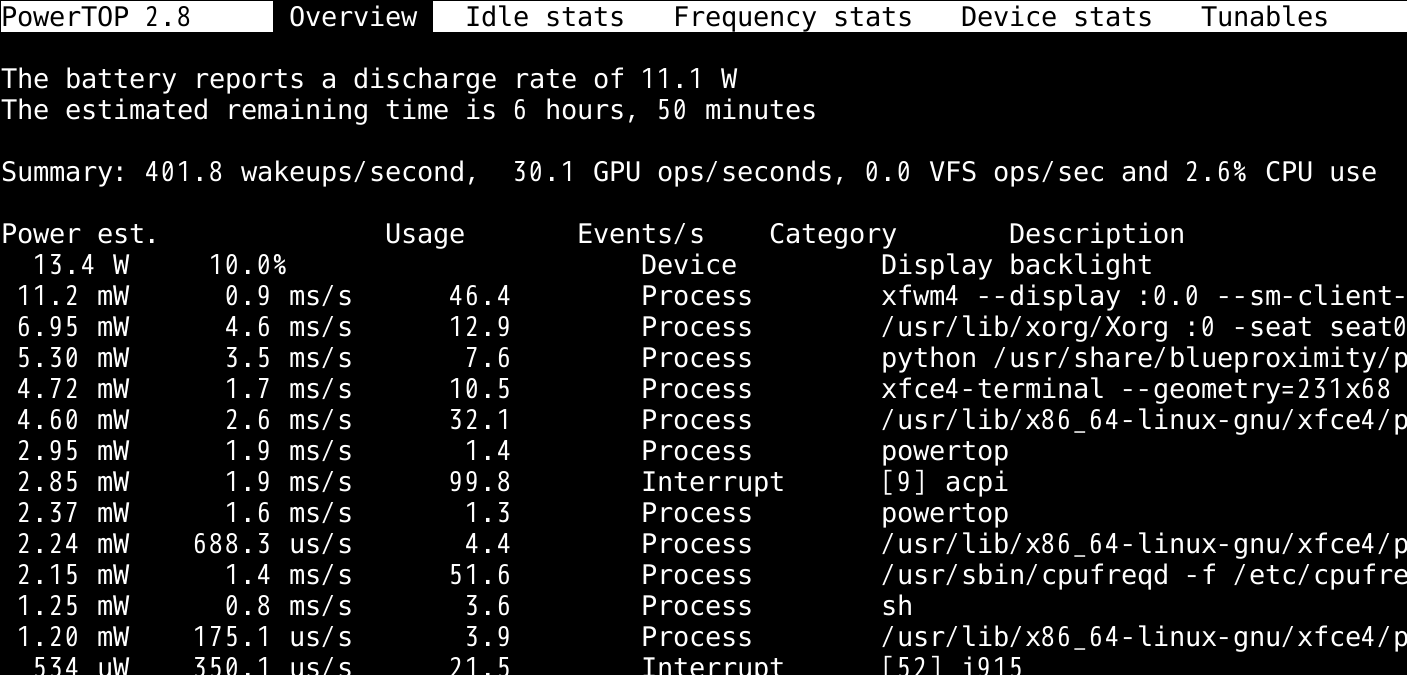
\includegraphics[width=0.5\hsize]{image201602/powertop_02.png}
\end{center}
\label{fig:powertop2}
\caption{省電力設定後} 
\end{figure}

\subsection{まとめ}

Debian での省電力設定について説明しました。
現在の状態をとりあえず確認するには cpufreq-info を使い、カーネルの設定やドライバの設定は
sysfs や proc fs 経由で設定します。プログラムやプロセスの詳細な状態の確認するには PowerTOP
を使います。省電力設定できる項目もわかり、ユーザインターフェイスから各種設定ができるようになっています。
また再立ち上げすると省電力設定を再設定する必要がありますので、sysytem用のservice
ファイルを別途用意するなどの対策が必要です。
細かい設定を行わなくても、とりあえず省電力設定を行いたい場合はTLPを使うのがよいでしょう。ただ全ての
PCをサポートしているわけではありませんので、環境に合わせてプログラムを修正するなりの対応が必要となります。

\if0
%-------------------------------------------------------------------------------
\dancersection{会場での無線LANのつなぎ方}{野島 貴英,Roger}
%-------------------------------------------------------------------------------
 \subsection{はじめに}

 今回会場側には無線LAN経由のグローバル回線が用意されています。

 以下にDebianマシンでの接続方法を記載します。

 また、自分の環境では違うやり方でつながったという方は、野島まで
教えて下さい。こちらでもノウハウとして溜めていく予定です。

 \subsection{wpasupplicant及び/etc/network/interfacesを利用の場合}

 もっとも良いマニュアルは、/usr/share/doc/wpasupplicant/README.Debian.gz
となります。困った場合はこちらも合わせてご参照下さい。

 以下に/etc/network/interfacesの定義について会場の例を記載します。

\begin{commandline}
$ sudo vi /etc/network/interfaces
-----以下のエントリがなければ追記ここから----------
iface wlan0_debian inet dhcp
     wpa-conf /etc/wpa_supplicant/wpa_supplicant_debian.conf
-----以下のエントリがなければ追記ここまで----------
$ sudo vi /etc/wpa_supplicant/wpa_supplicant_debian.conf
-----以下のエントリを追記ここから----------
network={
     ssid=<<会場のSSID>>
     psk=<<会場のパスワード>>
     scan_ssid=1
}
-----以下のエントリを追記ここまで----------
$ sudo chmod 600 /etc/wpa_supplicant/wpa_supplicant_debian.conf
$ sudo ifup wlan0=wlan0_debian
\end{commandline}
%$

 また、ハマってしまった時のデバッグ方法は、
/usr/share/doc/wpasupplicant/README.Debian.gz中の''4. Trubleshooting''の章が便利です。

 \subsection{その他の無線LAN用パッケージを利用の場合}

 すみません、自分が情報を持たないため、現場で教えて下さい。

\fi

\cleartooddpage

\vspace*{15cm}
\hrule
\vspace{2mm}

\includegraphics[width=2cm]{image200502/openlogo-nd.eps}
\noindent \Large \bf Debian 勉強会資料\\
\noindent \normalfont \debmtgyear{}年\debmtgmonth{}月\debmtgdate{}日 \hspace{5mm}  初版第1刷発行\\
\noindent \normalfont 東京エリア Debian 勉強会 (編集・印刷・発行)\\
\hrule

\end{document}
